\documentclass{beamer}
\usepackage[utf8]{inputenc}
\usepackage{xeCJK} 
\usepackage[T1]{fontenc}
\usepackage{mathabx}
\usepackage{amsmath} 
\usepackage{mathpazo}
\usepackage{bibentry}
\usepackage{tikz}
\usepackage{caption}
\usepackage{graphicx, subfig}

\usetikzlibrary{scopes}
\def\iangle{35} % Angle of the inclined plane
\def\down{-90}
\def\arcr{0.5cm} % Radius of the arc used to indicate angles

\usetheme{Boadilla}
\usecolortheme{wolverine}
\useoutertheme{miniframes}

\title{VP160 Recitation Class V}
% \subtitle{Non-inertial FoR}
\author{Zeyi Ren}
\institute{UM-SJTU Joint Institute}

\begin{document}

\maketitle

%\frame{\tableofcontents}
\section{Work}
\begin{frame}{Work}
  \begin{block}{Definition}
    \begin{equation}\delta W = \vec{F}\circ d\vec{r}\end{equation}
    \begin{equation}
    W_{AB}=\int_{\Gamma_{A B}} \vec{F}\circ d\vec{r} 
    \end{equation}
    \begin{center}In general, $\vec{F} = \vec{F}(\vec{r})$ (position-dependent force; vector field)\end{center}
  \end{block}
  \pause
  ~\\
  \textcolor{blue}{Methods for Calculation}\\
\begin{enumerate}
  \item Constant force on a straight line
  \item Varying force on a straight line (Integral)
  \item Varying force on a curve (Line integral)
\end{enumerate}
\end{frame}

\begin{frame}
\textcolor{blue}{Exercise 1}

Find work done by the force $\mathbf{F_1}(x,y) = -x\hat{n_x} -y\hat{n_y}$ and by the force $\mathbf{F_2}(x,y) = (2xy + y)\hat{n_x} + (x^2 + 1)\hat{n_y}$ if a particle is being moved from $(-1, 0)$ to $(0, 1)$ along\\
(a) the straight line connecting these points,\\
(b) the (shorter) arc of the circle $x^2 + y^2 = 1$,\\
(c) the axes of the Cartesian coordinate system: first from $(-1, 0)$ to $(0, 0)$ along the $x$ axis, then from $(0, 0)$ to $(0, 1)$ along the $y$ axis.
\end{frame}

\section{Kinetic Energy and Power}
\begin{frame}
  Recall that $\delta W = \vec{F}\circ d\vec{r}$, so the rate of work being done by the net force on a particle 
  $$
  \frac{\delta W}{dt} = \vec{F}\circ \frac{d\vec{r}}{dt}=\vec{F}\circ \vec{v} = m \dot{\vec{v}}\circ \vec{v}=\frac{d}{dt}(\frac{1}{2}mv^2) 
  $$
  \pause
  \begin{itemize}
    \item \textcolor{blue}{Kinetic Energy}:$E_k=\frac{1}{2}mv^2$
    \item \textcolor{blue}{Work-Kinetic Energy Theorem}: $\delta W = dE_k$\pause
    \item \textcolor{blue}{Average Power}:$P_{av}=\frac{W}{\Delta t}$
    \item \textcolor{blue}{Instantaneous power}:$P_{ins} = \frac{\delta W}{dt}=\vec{F}\circ \vec{v}$
  \end{itemize}
\end{frame}

\section{Conservative Forces and Potential Energy}
\begin{frame}{Conservative Force}
  \begin{itemize}
    \item Path-Independent.
    \begin{itemize}
      \item If $\vec{F}$ is conservative $\Rightarrow \Delta W_{AB} = Constant$\pause
      \item e.g. Gravitational Force, Elastic Force 
    \end{itemize}\pause
    \item How to determine?
    \begin{itemize}
      \item In a simple connected region, $rot\vec{F} = 0$ $$\begin{aligned}
        \operatorname{rot} \vec{F}=&\left|\begin{array}{ccc}
        \hat{n}_{x} & \hat{n}_{y} & \hat{n}_{z} \\
        \frac{\partial}{\partial x} & \frac{\partial}{\partial y} & \frac{\partial}{\partial z} \\
        F_{x} & F_{y} & F_{z}
        \end{array}\right|\\=&  \hat{n}_{x}\left(\frac{\partial F_{z}}{\partial y}-\frac{\partial F_{y}}{\partial z}\right)+\hat{n}_{y}\left(\frac{\partial F_{x}}{\partial z}-\frac{\partial F_{z}}{\partial x}\right)+\hat{n}_{z}\left(\frac{\partial F_{y}}{\partial x}-\frac{\partial F_{x}}{\partial y}\right)=0
        \end{aligned}$$\pause
        % $$\Rightarrow \frac{\partial F_{z}}{\partial y}=\frac{\partial F_{y}}{\partial z},\quad \frac{\partial F_{x}}{\partial z}=\frac{\partial F_{z}}{\partial x},\quad \frac{\partial F_{y}}{\partial x}=\frac{\partial F_{x}}{\partial y}$$
        \item Relation with Potential Energy:$$\vec{F}=-\bigtriangledown U=-\frac{\partial U}{\partial x}\hat{n_x}-\frac{\partial U}{\partial y}\hat{n_y}-\frac{\partial U}{\partial z}\hat{n_z}$$
    \end{itemize}\pause
    \item Non-conservative force?
  \end{itemize}
\end{frame}

\begin{frame}
\textcolor{blue}{Exercise 2}

Consider a 3D force $$ \vec{F}=\left(\begin{array}{c}
  6xyz^2+3y^2\\
  3x^2y^2+6xy-z\\
  6x^2yz-y
  \end{array}\right)$$
  Is it a conservative force? How to find the corresponding potential energy?
\end{frame}

\section{Conservation of the Total Energy}
\begin{frame}
  The net force may be the sum of a conservative force and a non-conservative force$$\vec{F}=\vec{F}_{con}+\vec{F}_{\text {n-cons}}$$\pause
   The work done by the net force (by \textbf{Work-Kinetic Energy Theorem}):
$$
\delta W=\vec{F} \circ d \vec{r}=\vec{F}_{con } \circ d \vec{r}+\vec{F}_{\text {n-cons}} \circ d\vec{r} =d K
$$\pause
However, only for conservative force $\vec{F}_{con} \circ d \vec{r}=-d U$. Hence, the elementary work done by the non-conservative force is
$$
\delta W_{\text {n-cons}}=\vec{F}_{\text {n-cons}} \circ d \vec{r}=d(K+U)
$$\pause
and the total work done from $A$ to $B$
$$
W_{\text {n-cons}}=\int_{\Gamma_{A B}} \vec{F}_{\text {n-cons}} \circ d\vec{r}=E(B)-E(A)=\Delta E = -\Delta U_{int}
$$\pause
and we finally get the \textbf{Law of Conservation of the Total Energy}:
$$
\Delta\mathbf{K} + \Delta \mathbf{U} +\Delta \mathbf{U_{int}} = 0
$$
\end{frame}

\begin{frame}{Energy Diagram}
  \begin{figure}[htbp]
  \centering
  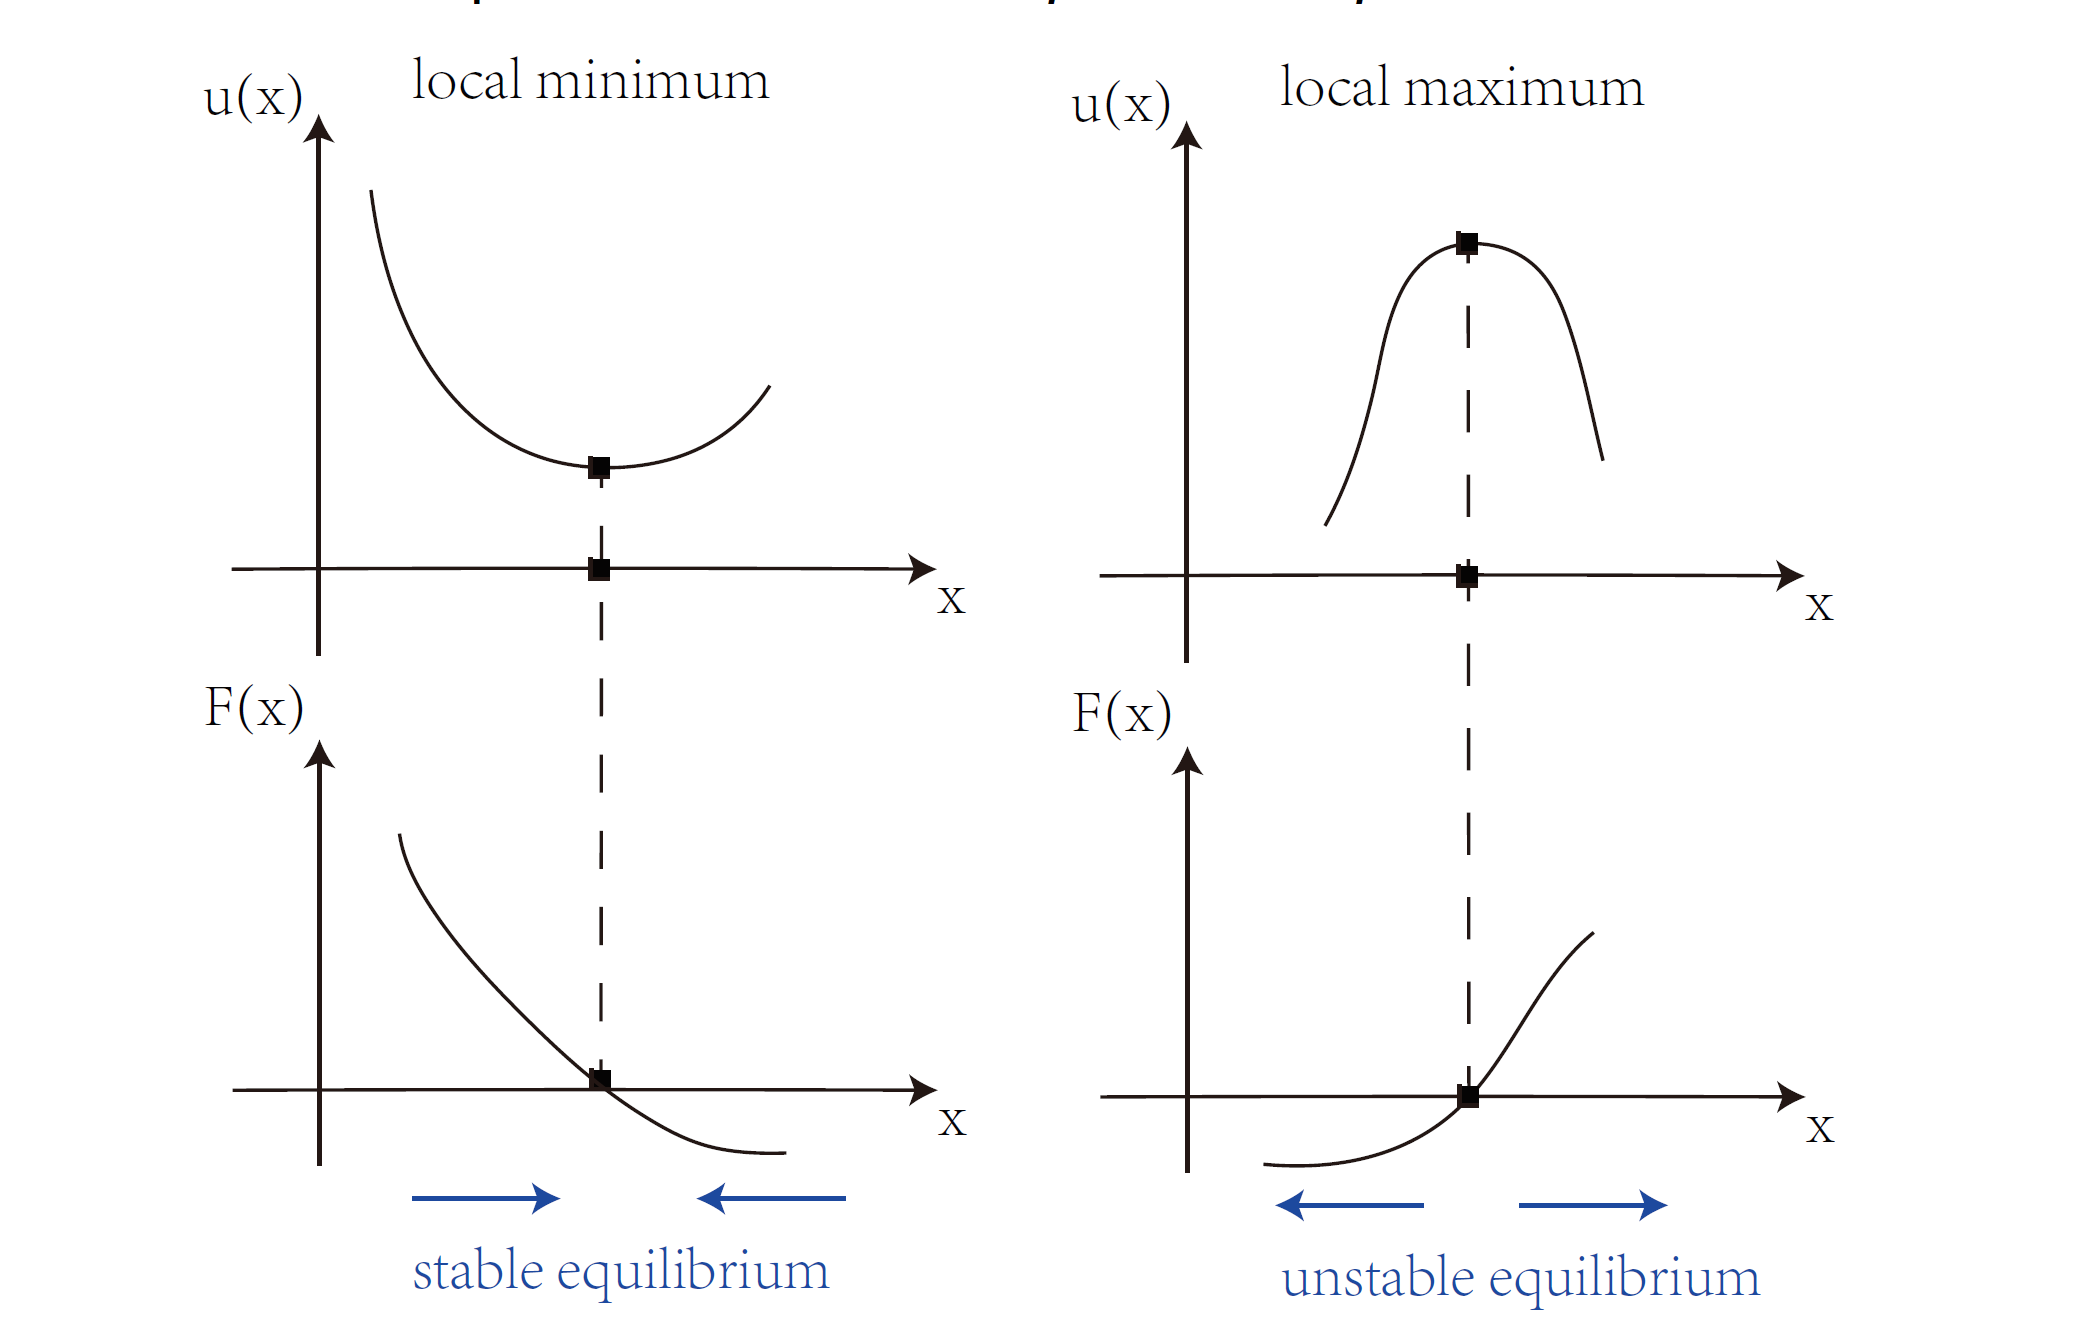
\includegraphics[width= 0.9\linewidth, angle =0]{EnergyDiagram.png}
  % \caption{.}
  \label{fig:1}
  \end{figure}
\end{frame}

\begin{frame}{Reference}
  \begin{thebibliography}{9}
  \setbeamertemplate{bibliography item}[article]
  \bibitem{C} Yigao Fang.\\
  \textcolor{black}{VP160 Recitation Slides.}\\
  2020
  \bibitem{C} Haoyang Zhang.\\
  \textcolor{black}{VP160 Recitation Slides.}\\
  2020
  \setbeamertemplate{bibliography item}[book]
  \bibitem{C} Yousheng Shu (舒幼生).\\
  \textcolor{black}{\textit{Mechanics (力学)}}\\
  Peking University Press, 2005
  % \setbeamertemplate{bibliography item}[book]
  % \bibitem{C} Jiafu Cheng (程稼夫).\\
  % \textcolor{black}{\textit{中学奥林匹克竞赛物理教程:力学篇}}\\
  % University of Science and Technology Press, 2013
  \end{thebibliography}
  \end{frame}
  \end{document}



